\section{Безопасность IOT}
Каждое подключенное устройство создает возможности для \\злоумышленников. Эти уязвимости обширны, даже
для одного небольшого устройства. Векторы угроз представлены на рисунке  \ref{fig:section7:security_issues} Представляемые риски включают передачу данных, доступ к устройству, неисправность
устройства, а также постоянно включенные/всегда подключенные устройства.\cite{DeisgOfIOT}
\begin
{figure}[h!]
    \centering
    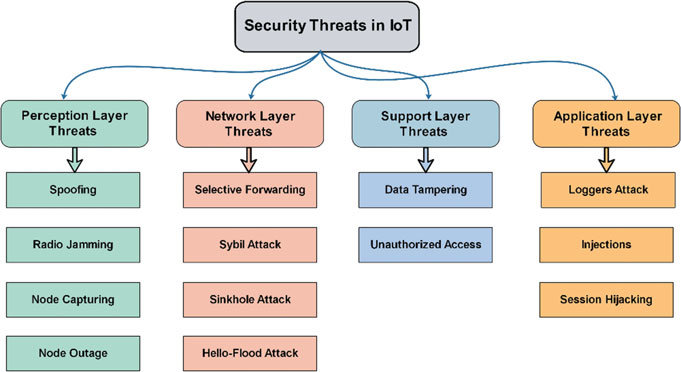
\includegraphics[scale=0.6]{security_issues.png}
    \caption{Возможные угрозы на разных уровнях представления}
    \label{fig:section7:security_issues}
\end{figure}

Основными проблемами в области безопасности остаются ограничения безопасности, связанные с производством недорогих устройств, и растущее количество устройств, создающее больше возможностей для атак.

Помимо затрат и повсеместного распространения устройств, IoT мешают другие проблемы безопасности:
\begin{itemize}
    \item Непредсказуемое поведение — огромное количество развернутых устройств и их длинный список
    обеспечивающие технологии означают, что их поведение в полевых условиях может быть непредсказуемым. Специфический
    система может быть хорошо спроектирована и находиться под административным контролем, но нет
    гарантии того, как он будет взаимодействовать с другими.

    \item Сходство устройств — устройства IoT довольно однородны. Они используют одно и то же соединение
    технологии и компоненты. Если одна система или устройство подвержены уязвимости, многие
    у многих такая же проблема.

    \item Проблемное развертывание. Одной из основных целей IoT остается размещение передовых
    сети и аналитика там, где раньше они не могли пройти. К сожалению, это создает
    проблема физической защиты устройств в этих странных или легкодоступных местах.
    
    \item Длительный срок службы устройства и просроченная поддержка. Одним из преимуществ устройств IoT является
    долговечность, однако этот долгий срок службы также означает, что они могут прожить дольше, чем срок поддержки этих устройств.
    Сравните это с стандартными системами, которые, как правило, имеют поддержку и обновления спустя долгое время.
    Устройства без обновлений и поддержки ПО не имеют того же самого
    усовершенствования систем безопасности, в связи с развитием технологий с течением времени.
    
    \item Отсутствие поддержки обновлений. Многие устройства IoT, как и многие мобильные и небольшие устройства, либо сложны в поддержке, либо не поддерживаются.
    Остальные же предлагают неудобные способы обновления, которые многие владельцы игнорируют или не замечают.
    
    \item Низкая прозрачность или отсутствие прозрачности. Многие устройства IoT не обеспечивают прозрачность в отношении
    к их функциональности. ользователи не могут наблюдать за существующеми процессами, а так же не могут получить полный доступ к своим же устройствам. У них нет контроля над зловредными функциями, которые могут отправлять даные на промежуточные сервера. Кроме того, когда производитель обновляет устройство, это может принести еще больше
    проблем на уровне ПО.
    
    \item Отсутствие предупреждений об отказах и ошибках. Другой целью Интернета вещей остается обеспечение его обширной функциональности без навязчивости к конечному пользователю. Это приводит к проблеме неосведомленности пользователей. Пользователи не следят за состоянием
    устройства и, соотвественно, не могут узнать узнать, когда с ним что-то пойдет не так. Ошибки в коде, которые приводят к пробеме безопасности могут сохраняться в течение длительного времени без обнаружения и испрвления.
\end{itemize}